\documentclass[tikz,border=0pt]{standalone}
% Shared publication style. Compile figure sources from this directory.
\usepackage[T1]{fontenc}
\usepackage{lmodern}
\usepackage{amsmath,amssymb}
\usepackage{tikz}
\usepackage{pgfplots}
\usetikzlibrary{arrows.meta,calc,positioning,backgrounds,patterns,shapes.geometric}
\usepgfplotslibrary{groupplots,fillbetween}
\pgfplotsset{compat=1.18}
\definecolor{fgblue}{HTML}{0072B2}
\definecolor{fgorange}{HTML}{D55E00}
\definecolor{fgslate}{HTML}{8B949E}
\definecolor{fgdark}{HTML}{25313C}
\definecolor{fgpale}{HTML}{F2F6F8}
\definecolor{fggrid}{HTML}{E3E8EC}
\definecolor{fgwater}{HTML}{D6EAF4}
\definecolor{fgland}{HTML}{E8E3D3}
\renewcommand{\familydefault}{\sfdefault}
\tikzset{every picture/.style={font=\fontsize{9}{11}\selectfont,text=fgdark},
  panel label/.style={font=\bfseries\fontsize{10}{12}\selectfont,anchor=north west},
  panel title/.style={font=\bfseries\fontsize{9}{11}\selectfont,anchor=north west},
  light arrow/.style={-{Stealth[length=1.6mm]},draw=fgslate,line width=.65pt}}
\pgfplotsset{fg axis/.style={
  axis line style={fgslate,line width=.4pt},axis x line*=bottom,axis y line*=left,
  tick align=outside,tick style={fgslate,line width=.4pt},
  tick label style={font=\fontsize{8}{10}\selectfont,text=fgdark},
  label style={font=\fontsize{9}{11}\selectfont,text=fgdark},
  title style={font=\bfseries\fontsize{9}{11}\selectfont,text=fgdark},
  grid style={fggrid,line width=.35pt},minor tick num=0,
  legend style={draw=none,fill=none,font=\fontsize{8}{10}\selectfont},
  scaled ticks=false,clip=false,
  every axis plot/.append style={line width=.85pt,mark size=2.2pt}
}}

% Reported values from tex/main.tex lines 1399,1444 and
% reports/fisher_glass_results_report.md (Synthetic and Tail Boundary).
% A single-seed point estimates; B and C five-seed mean +/- 1.96 SE.
\begin{document}
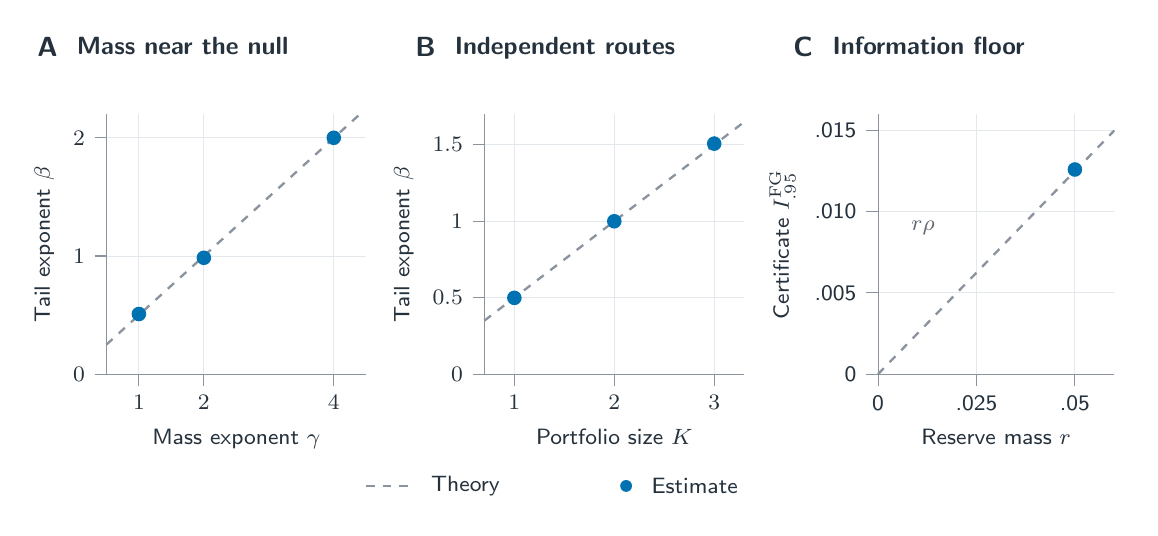
\begin{tikzpicture}[x=1mm,y=1mm]
\path[use as bounding box] (0,0) rectangle (140,61);
\node[panel label] at (0,61) {A};
\node[panel title] at (5,61) {Mass near the null};
\node[panel label] at (48,61) {B};
\node[panel title] at (53,61) {Independent routes};
\node[panel label] at (96,61) {C};
\node[panel title] at (101,61) {Information floor};
\begin{axis}[fg axis,at={(10mm,17mm)},anchor=south west,width=33mm,height=33mm,scale only axis,
 xmin=.5,xmax=4.5,ymin=0,ymax=2.2,xtick={1,2,4},ytick={0,1,2},grid=major,
 xlabel={Mass exponent $\gamma$},xlabel style={font=\fontsize{8}{10}\selectfont},
 ylabel={Tail exponent $\beta$},ylabel style={font=\fontsize{8}{10}\selectfont}]
\addplot[fgslate,dashed,domain=.5:4.4] {x/2};
\addplot[only marks,mark=*,fgblue] coordinates {(1,.509) (2,.985) (4,2.001)};
\end{axis}
\begin{axis}[fg axis,at={(58mm,17mm)},anchor=south west,width=33mm,height=33mm,scale only axis,
 xmin=.7,xmax=3.3,ymin=0,ymax=1.7,xtick={1,2,3},ytick={0,.5,1,1.5},grid=major,
 xlabel={Portfolio size $K$},xlabel style={font=\fontsize{8}{10}\selectfont},
 ylabel={Tail exponent $\beta$},ylabel style={font=\fontsize{8}{10}\selectfont}]
\addplot[fgslate,dashed,domain=.7:3.3] {x/2};
\addplot[only marks,mark=*,fgblue,error bars/.cd,y dir=both,y explicit,error bar style={line width=.7pt},error mark options={mark size=2pt}]
 coordinates {(1,.499) +- (0,.003) (2,1.000) +- (0,.009) (3,1.508) +- (0,.015)};
\end{axis}
\begin{axis}[fg axis,at={(108mm,17mm)},anchor=south west,width=30mm,height=33mm,scale only axis,
 xmin=0,xmax=.06,ymin=0,ymax=.016,xtick={0,.025,.05},xticklabels={0,.025,.05},
 ytick={0,.005,.01,.015},yticklabels={0,.005,.010,.015},grid=major,
 xlabel={Reserve mass $r$},xlabel style={font=\fontsize{8}{10}\selectfont},
 ylabel={Certificate $I^{\mathrm{FG}}_{.95}$},ylabel style={font=\fontsize{8}{10}\selectfont}]
\addplot[fgslate,dashed,domain=0:.06] {x*.25};
\addplot[only marks,mark=*,fgblue,error bars/.cd,y dir=both,y explicit,error mark options={mark size=2pt}]
 coordinates {(.05,.0126) +- (0,.000001)};
\node[anchor=west,font=\fontsize{8}{10}\selectfont,text=fgslate!70!black] at (axis cs:.006,.009) {$r\rho$};
\end{axis}
\draw[fgslate,dashed,line width=.85pt] (43,2.8)--(49,2.8);
\node[anchor=west,font=\fontsize{8}{10}\selectfont] at (50,2.8) {Theory};
\fill[fgblue] (76,2.8) circle (.75);
\node[anchor=west,font=\fontsize{8}{10}\selectfont] at (78,2.8) {Estimate};
\end{tikzpicture}
\end{document}
